\documentclass[conference,10pt,letterpaper]{IEEEtran}
\usepackage[T1]{fontenc}
\usepackage{tgtermes}
\pdfmapfile{+qtm.map}
\usepackage{etoolbox}
\usepackage{amsmath,amssymb,graphicx,booktabs,array,microtype,tikz,url,float,tabularx}
\graphicspath{{../}{./}}
\usetikzlibrary{arrows.meta,positioning}
\usepackage[hidelinks]{hyperref}
\hypersetup{pdftitle={IITK Report},pdfauthor={nojobsforus, IIT Roorkee}}
\setlength{\textfloatsep}{7pt plus 1pt minus 1pt}
\setlength{\intextsep}{7pt plus 1pt minus 1pt}
\setlength{\floatsep}{6pt plus 1pt minus 1pt}
\newcommand{\attack}[1]{\textbf{#1}}
\patchcmd{\subsection}{\itshape}{\upshape}{}{\errmessage{Subsection font patch failed}}
\patchcmd{\subsubsection}{\itshape}{\upshape}{}{\errmessage{Subsubsection font patch failed}}
\patchcmd{\abstract}{\textit}{\textbf}{}{\errmessage{Abstract font patch failed}}
\patchcmd{\abstract}{---}{:\ }{}{\errmessage{Abstract separator patch failed}}

\begin{document}
\title{IITK INNOVATION CHALLENGE 2026 Qualification Report\\[1.1ex]
\large\textbf{yuri daisuki - IIT Roorkee}}
\author{\normalsize\setlength{\tabcolsep}{3pt}\begin{tabular}{ccc}
\begin{tabular}{c}{\large Taufeeque Sifat}\\taufeeque\_as@ce.iitr.ac.in\\\text{IIT Roorkee}\end{tabular}&
\begin{tabular}{c}{\large Shivam}\\shivam1@me.iitr.ac.in\\\text{IIT Roorkee}\end{tabular}&
\begin{tabular}{c}{\large Divyam Kumar}\\divyam\_k@ee.iitr.ac.in\\\text{IIT Roorkee}\end{tabular}\\[6ex]
\multicolumn{3}{c}{\begin{tabular}{cc}
\end{tabular}}
\end{tabular}}
\maketitle
\raggedbottom

\begin{abstract}
This report analyzes power traces from an AES-128 implementation to recover a countermeasure-induced fake round-10 key, estimate the trace count required for its recovery, infer the actual round-10 key, and derive the AES-128 master key. For fake key recovery, correlation power analysis (CPA) is applied using a transition Hamming-distance leakage hypothesis over ciphertext bytes and trace samples. trace count performance is measured by ranking each reference key byte as the number of traces varies. The first tested trace count at which all 16 reference bytes reach rank 1 is 1,933; rank 1 is then maintained for 100 consecutive tested counts beginning at 2,020. To infer the actual round-10 key, the analysis identifies absent ciphertext byte values, detects round activity from across-trace variance, and ranks shared missing S-box input candidates using transition-leakage correlations for rounds 1--8. The selected candidate is $z=\texttt{0xFF}$, yielding the round-10 key \texttt{d014f9a8c9ee2589e13f0cc8b6630ca6}. Reversing the AES-128 key schedule gives the master-key candidate \texttt{2b7e151628aed2a6abf7158809cf4f3c}. The actual round-key inference depends on the shared-endpoint and leakage-model assumptions used in the candidate scan.
\end{abstract}

\section{Introduction}
Power consumption can vary with the data a processor reads, writes, and transforms. A power trace therefore contains information about internal computation, even when the cryptographic output alone does not reveal it. Side-channel analysis uses a model of that computation to compare predicted intermediate values with measurements. Correlation power analysis (CPA) is one way to rank key guesses by how closely their predicted leakage follows the recorded traces \cite{kocher,brier}.

This report studies a trace challenge, with the premise being an AES-128 implementation on an embedded device and its power traces for the 10th round provided to us, along with four related tasks. There is a faking countermeasure as well, which aims to protect the implementation against conventional CPA, with one such countermeasure defined in~\cite{faking}.

The first asks for a fake round-10 key from the final-round leakage. The second asks how the number of traces affects recovery of that key and to report the minimum number of traces for effective recovery fo the fake key. The third asks for the actual round-10 key, despite the fake key behavior at the final round. The fourth asks for the AES-128 master key. The analysis uses CPA for the first two tasks, then combines ciphertext-frequency observations with leakage from earlier AES rounds for the third. The final task reverses the AES-128 key schedule \cite{fips197}.

Side-channel based reverse engineering uses physical leakage to infer internal algorithm or implementation details. Novak studies this use of side channels through sign-extended differential power analysis and attacks on table lookups~\cite{novak-reverse}. Task 3 fits within this broader category because we use ciphertext statistics and power traces to test hypotheses about the faking countermeasure. Here, we know that the device uses AES; the inference concerns the countermeasure's lookup-table behavior and the actual round key.

The fake key attack uses a transition Hamming-distance hypothesis and searches all 200 samples for each key-byte guess. For the trace count study, the byte ranks are recomputed on prefixes of one seeded shuffle of the capture. For the actual round-10 key, the analysis first finds ciphertext byte values that are absent from the capture, then tests the corresponding endpoint candidates against transition leakage at detected round-activity samples. The selected round key is reversed through the AES-128 key schedule to obtain a master-key candidate.

The results support the fake round-10 key \texttt{91dec068e3face4599ce38f420863a30}. In the saved trace count characterization, all 16 bytes first reach rank 1 at 1,933 traces; they then remain at rank 1 for 100 successive tested counts beginning at 2,020. The selected actual round-10 key is \texttt{d014f9a8c9ee2589e13f0cc8b6630ca6}, and its reversed master-key candidate is \texttt{2b7e151628aed2a6abf7158809cf4f3c}. The actual-key result is evidence under the leakage and shared-endpoint assumptions described below, rather than a proof independent of those assumptions.

Section II reviews the AES and leakage-model details needed for the analysis. Section III describes the trace data and experimental settings. Section IV gives the method used for each task, and Section V presents the results. Section VI discusses limitations, followed by the conclusion in Section VII.

Figure~\ref{fig:variance} gives the variance profile used to locate round activity in the traces.

\begin{figure*}[!t]
\centering
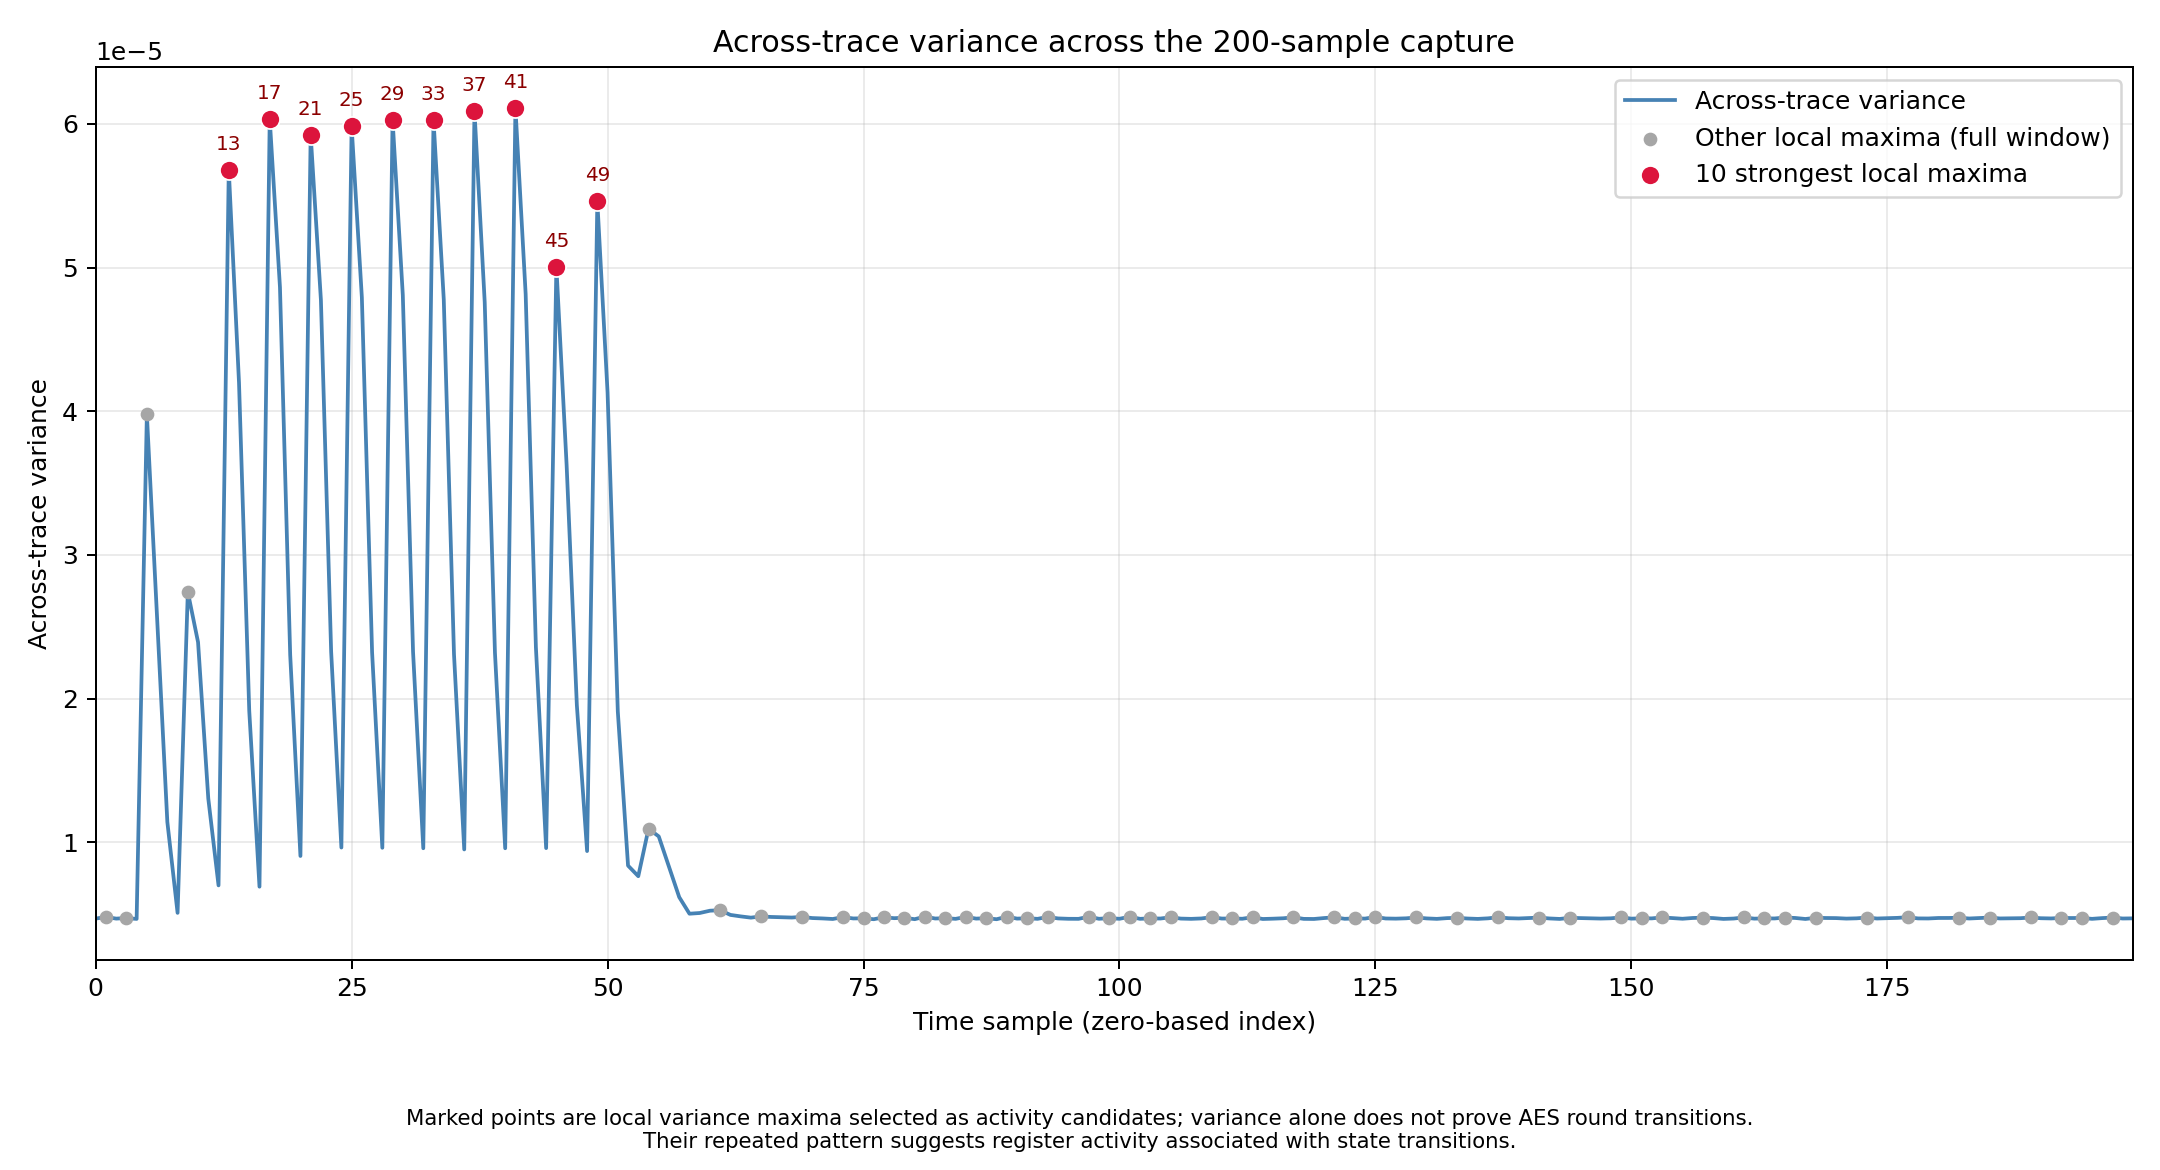
\includegraphics[width=0.92\textwidth]{variance_plot.png}
\caption{Across-trace variance over the 200-sample capture. The selected local maxima indicate candidate activity times.}
\label{fig:variance}
\end{figure*}

\section{Background and Problem Formulation}
\subsection{AES-128 and the Round-10 Key}
AES-128 encrypts a 128-bit block using an initial key addition followed by ten rounds. The AES-128 key schedule expands the 128-bit master key into eleven 128-bit round keys. The final ciphertext is produced by the tenth round and its round key, commonly denoted $RK_{10}$ \cite{fips197}. Because the key schedule is reversible, a candidate $RK_{10}$ determines a candidate master key.

The challenge's final-round leakage is associated with a fake key. Consequently, applying a final-round CPA model can recover the fake key without directly revealing the actual $RK_{10}$. Tasks 3 and 4 use ciphertext statistics and leakage associated with earlier rounds to pursue the actual round key and then the master key.

\subsection{Leakage Model and CPA}
The analysis assumes first-order leakage related to the Hamming distance (HD) between two byte values. For a byte value $x$, its Hamming weight, $HW(x)$, is the number of set bits. A transition from $x$ to $y$ is modeled by $HW(x\oplus y)$, where $\oplus$ denotes XOR. This is a simplified leakage model. Real measurements can also contain noise, unrelated activity, and effects not captured by the model.

For Task 1, let $C_{j,b}$ be ciphertext byte $b$ for trace $j$, and let $\pi(b)$ identify the ciphertext byte routed to the corresponding pre-output state position by the AES ShiftRows mapping. For key guess $k$, the predicted final-round transition is
\begin{equation}
H_{j,b}(k)=HW\!\left(\operatorname{InvSBox}(C_{j,b}\oplus k)\oplus C_{j,\pi(b)}\right).
\label{eq:task1-hypothesis}
\end{equation}
For a hypothesis vector $H_b(k)$ and the measured vector $P(t)$ at sample $t$, the Pearson correlation is~\cite{oflynn2014}
\begin{equation}
\begin{aligned}
&\rho\big(H_b(k),P(t)\big)\\
&\quad=\frac{\displaystyle\sum_{j=1}^{n}\big(H_{j,b}(k)-\overline{H}_{b,k}\big)\big(P_j(t)-\overline{P}_t\big)}
{\displaystyle\sqrt{\sum_{j=1}^{n}\big(H_{j,b}(k)-\overline{H}_{b,k}\big)^2}\,
\displaystyle\sqrt{\sum_{j=1}^{n}\big(P_j(t)-\overline{P}_t\big)^2}},
\end{aligned}
\label{eq:pearson}
\end{equation}
where $n$ is the number of traces, $\overline{H}_{b,k}$ is the mean predicted leakage for guess $k$, and $\overline{P}_t$ is the mean measured value at sample $t$. The correlation is the centered covariance divided by the product of the two centered vector norms.
The guess score is the largest absolute value of Pearson correlation over the 200 trace samples:
\begin{equation}
S_b(k)=\max_{t\in\{0,\ldots,199\}}\left|\rho\big(H_b(k),P(t)\big)\right|,
\label{eq:task1-score}
\end{equation}
where $P(t)$ is the vector of measured values at sample $t$ across traces. The most-correct byte guess maximizes $S_b(k)$.

\subsection{Recovering the actual master key}
Since AES-128 key round schedule is reversible, getting the round-10 key will help in getting the initial AES master key. Let assume that expanded key is a 44 word , 4 bytes for each word, $w[0], w[1], \ldots,w[43]$~\cite{cse-inversion}. The first four words form the master key, while the last four form the round-10 key. The subsequent keys, after the master key, are calculated using a recurrence relation,
\begin{equation}
w[i]=w[i-4]\oplus F_i(w[i-1]),
\label{eq:forward-schedule}
\end{equation}
At every fourth word, $F_i$ applies byte rotation, the forward S-box, and the round constant while at other positions, it leaves its input unchanged. Mathematically:
\begin{equation}
F_i(x)=
\begin{cases}
\begin{aligned}
&\operatorname{SubWord}(\operatorname{RotWord}(x))\\
&\quad\oplus Rcon[i/4],
\end{aligned}
& i\equiv0\pmod4,\\
x, & \text{otherwise}.
\end{cases}
\label{eq:schedule-transform}
\end{equation}
Here, the rotation, $\operatorname{RotWord}$, moves the first byte to the end of the four-byte word. The substitution, $\operatorname{SubWord}$, replaces each byte with its value from the forward AES S-box. The word $Rcon[r]$ contains the constant for round $r$ in its first byte and zeros in the remaining bytes~\cite{fips197}.

XORing both sides with $F_i(w[i-1])$ and setting $j=i-4$ gives backward rule to calculate previous round keys from the round-10 key~\cite{cse-inversion}:
\begin{equation}
w[j]=w[j+4]\oplus F_{j+4}(w[j+3]).
\label{eq:backward-schedule}
\end{equation}
Starting with $w[40],\ldots,w[43]$, we calculate $w[39]$ and continue backward to $w[0]$. Each step uses words that we already know. The resulting $w[0],\ldots,w[3]$ give the master key corresponding to the actual round-10 key.

\section{Dataset and Experimental Setup}
The capture in \texttt{Round10\_traces.csv} contains 100,000 records. Each record has a 16-byte ciphertext followed by 200 trace samples. Task 1 and Task 2 evaluate the CPA hypothesis over all 200 samples. Task 3 reads the capture directly, detects activity samples from across-trace variance, and excludes a row if any ciphertext byte equals the doubled value identified at that byte position. The remaining rows are used to reconstruct candidate AES states.

Task 2 uses NumPy's pseudorandom generator with seed \texttt{0x5CA} to permute the trace rows once. The fixed seed the shuffled ordering so that repeated runs use the same subsets and reproduce the experiment. This seed has no cryptographic value and does not affect the retrieval of the key, although different orderings can change the trace count required for recovery. It tests increasing prefixes, beginning at 250 traces, and records the rank of each byte of the full-data Task 1 key. The tested trace count stops after the worst byte rank has remained one for 100 consecutive counts, showing that the worst rank increases even after it has achieved the minimum value.

The scripts used for the analysis are \texttt{first\_task.py}, \texttt{second\_task.py}, \texttt{third\_task.py}, and \texttt{fourth\_task.py}. The trace count plots and table are saved in \texttt{rank\_plot\_all\_bytes.png}, \texttt{worst\_rank\_plot.png}, and \texttt{trace\_characterisation.csv}. Task 3 writes byte-wise candidate correlation plots to \texttt{actual\_round10\_correlation\_plots/}.

\section{Methodology}
\subsection{Task 1: Fake Round-10 Key Recovery}
For each of the 16 byte positions, the analysis evaluates all 256 byte key guesses. Equation~\eqref{eq:task1-hypothesis} gives the predicted transition leakage for a guess while Equation~\eqref{eq:task1-score} gives its score across the sample window. The key byte with the largest score is selected independently at each position. Concatenating the 16 winning bytes gives the fake round-10 key.

\subsection{Task 2: trace count Characterization}
The reference key is the 16-byte result of the Task 1 attack on the full-data. For each tested trace count $N$, the analysis uses the first $N$ rows from the fixed shuffled ordering and recomputes the CPA score for each byte guess using all 200 samples. For reference byte $F_b$, its rank is
\begin{equation}
r_b(N)=1+\left|\left\{k:S_{b,N}(k)>S_{b,N}(F_b)\right\}\right|,
\label{eq:rank}
\end{equation}
where $S_{b,N}(k)$ is the CPA score for guess $k$ using the first $N$ shuffled traces. The worst rank is $R(N)=\max_{0\leq b<16}r_b(N)$, so all bytes rank first exactly when $R(N)=1$.

The script reports two useful counts. The first full-recovery count is $\min\{N:R(N)=1\}$ over tested counts. The stable count is the first tested $N$ for which $R(N),R(N+1),\ldots,R(N+99)$ are all one. These values need not match because rankings can change as more traces are added.

\subsection{Task 3: Actual Round-10 Key Recovery}
For each ciphertext byte position, a histogram identifies an absent value $M_b$ and a most frequent (doubled) value $D_b$. Let $F_b$ be the fake key byte recovered in Task 1. Across all byte positions, the observed values satisfy
\begin{equation}
D_b\oplus F_b=SBox(0)=\texttt{0x63}.
\label{eq:doubled-fake-relation}
\end{equation}
This repeated relation connects the doubled ciphertext output to the Task 1 fake key and is consistent with a repeated lookup-table output associated with input zero. It describes the doubled values but does not identify the absent input or determine the actual round key by itself.

Trace timing is estimated separately from the key guesses. For sample $t$, across-trace variance is
\begin{equation}
V(t)=\frac{1}{N}\sum_{j=1}^{N}\left(P_j(t)-\overline{P}(t)\right)^2,
\qquad
\overline{P}(t)=\frac{1}{N}\sum_{j=1}^{N}P_j(t).
\label{eq:variance}
\end{equation}
The script finds local maxima of $V(t)$, selects the ten strongest, and places them in time order. In this capture they occur at samples 13, 17, 21, 25, 29, 33, 37, 41, 45, and 49. The four-sample spacing is consistent with repeated state-update activity. We use the first eight selected variance peaks to score the predicted state transitions for AES rounds 1-8. This assumes that the peaks correspond to successive rounds, which variance alone cannot confirm.

The shared-endpoint assumption is that the same missing S-box input $z$ explains the absent ciphertext output at all byte positions. Since the final AES round maps the relevant input through the S-box and XORs the round key, each candidate $z$ determines a candidate round key:
\begin{equation}
RK_{10,z}[b]=M_b\oplus SBox(z),\qquad z\in\{0,\ldots,255\}.
\label{eq:rk10-candidates}
\end{equation}
The candidate equation follows directly from the AES final-round byte relation. With no MixColumns in the last round, write the output at byte $b$ as
\begin{equation}
C_b=SBox(z_b)\oplus RK_{10}[b].
\label{eq:aes-final-byte}
\end{equation}
For an absent ciphertext value $M_b$, substitute $C_b=M_b$ in (\ref{eq:aes-final-byte}) and XOR both sides with $SBox(z_b)$. This gives
\begin{equation*}
RK_{10}[b]=M_b\oplus SBox(z_b).
\end{equation*}
The AES S-box is a permutation, so for a fixed round key and output byte there is exactly one corresponding input byte. The shared-endpoint hypothesis sets $z_b=z$ for all byte positions, yielding (\ref{eq:rk10-candidates}). Under the shared-$z$ assumption, the 256 possible values of $z$ give 256 candidate round keys. We use the power traces to rank these candidates.

For each candidate, the AES-128 schedule is reversed to obtain round keys, and standard AES states are reconstructed from the retained ciphertext rows. Predicted transition features are $H_{r,b}^{(z)}[j]=HW(S_{r-1}^{(z)}[j,b]\oplus S_r^{(z)}[j,b])$ for rounds 1-8 and retained trace $j$. At each detected event sample $t_r$, the code correlates this feature across traces with the measured sample vector. Its aggregate candidate score is
\begin{equation}
Q(z)=\frac{1}{8\cdot16}\sum_{r=1}^{8}\sum_{b=0}^{15}
\left|\rho\!\left(H_{r,b}^{(z)},P(t_r)\right)\right|.
\label{eq:endpoint-score}
\end{equation}
The candidate with the largest $Q(z)$ is selected.

\subsection{Task 4: Master-Key Recovery}
We use Equation~\eqref{eq:backward-schedule} to get the backward round keys from the recovered round-10 keys from Task 3.

The backward calculation still uses the forward S-box. We already know the input to $F_i$, so we can calculate its output using the usual rotation and substitution. The step that recovers the earlier word is the XOR in Equation~\eqref{eq:backward-schedule}. We therefore do not need to undo the S-box substitution when reversing the key schedule~\cite{fips197,cse-inversion}.

The round constants follow the rounds in reverse order. At $i=40,36,\ldots,4$, their first bytes are, in hexadecimal, \texttt{36, 1b, 80, 40, 20, 10, 08, 04, 02, 01}~\cite{fips197}. In \texttt{fourth\_task.py}, the list of constants follows the forward order, and its first entry has index zero. The script therefore uses entry $i/4-1$ to select the constant for a backward step. For example, $i=40$ selects entry 9, which contains \texttt{0x36}.

After the script reaches $w[0],\ldots,w[3]$, it joins those four words, keeping their original order, to form the master key candidate. To check the calculation, it runs the forward key schedule with this key and compares the resulting round-10 key with the input. A match confirms that the backward and forward calculations agree for the selected round key.

\section{Results and Discussion}
\subsection{Task 1: Fake Round-10 Key}
The full-data CPA selects the fake round-10 key
\begin{equation*}
\texttt{91\,de\,c0\,68\,e3\,fa\,ce\,45\,99\,ce\,38\,f4\,20\,86\,3a\,30}.
\end{equation*}
The winning peaks occur at sample 49 for most byte positions and at sample 50 for bytes 5 and 15. The per-byte peak absolute correlations range from approximately 0.119 to 0.178. Figure~\ref{fig:task1-example} shows byte 0 as an example; the remaining per-byte plots are supplied separately. The peak values are attack scores after searching 256 candidates over 200 samples, not statistical confidence bounds.

\begin{figure*}[t]
\centering
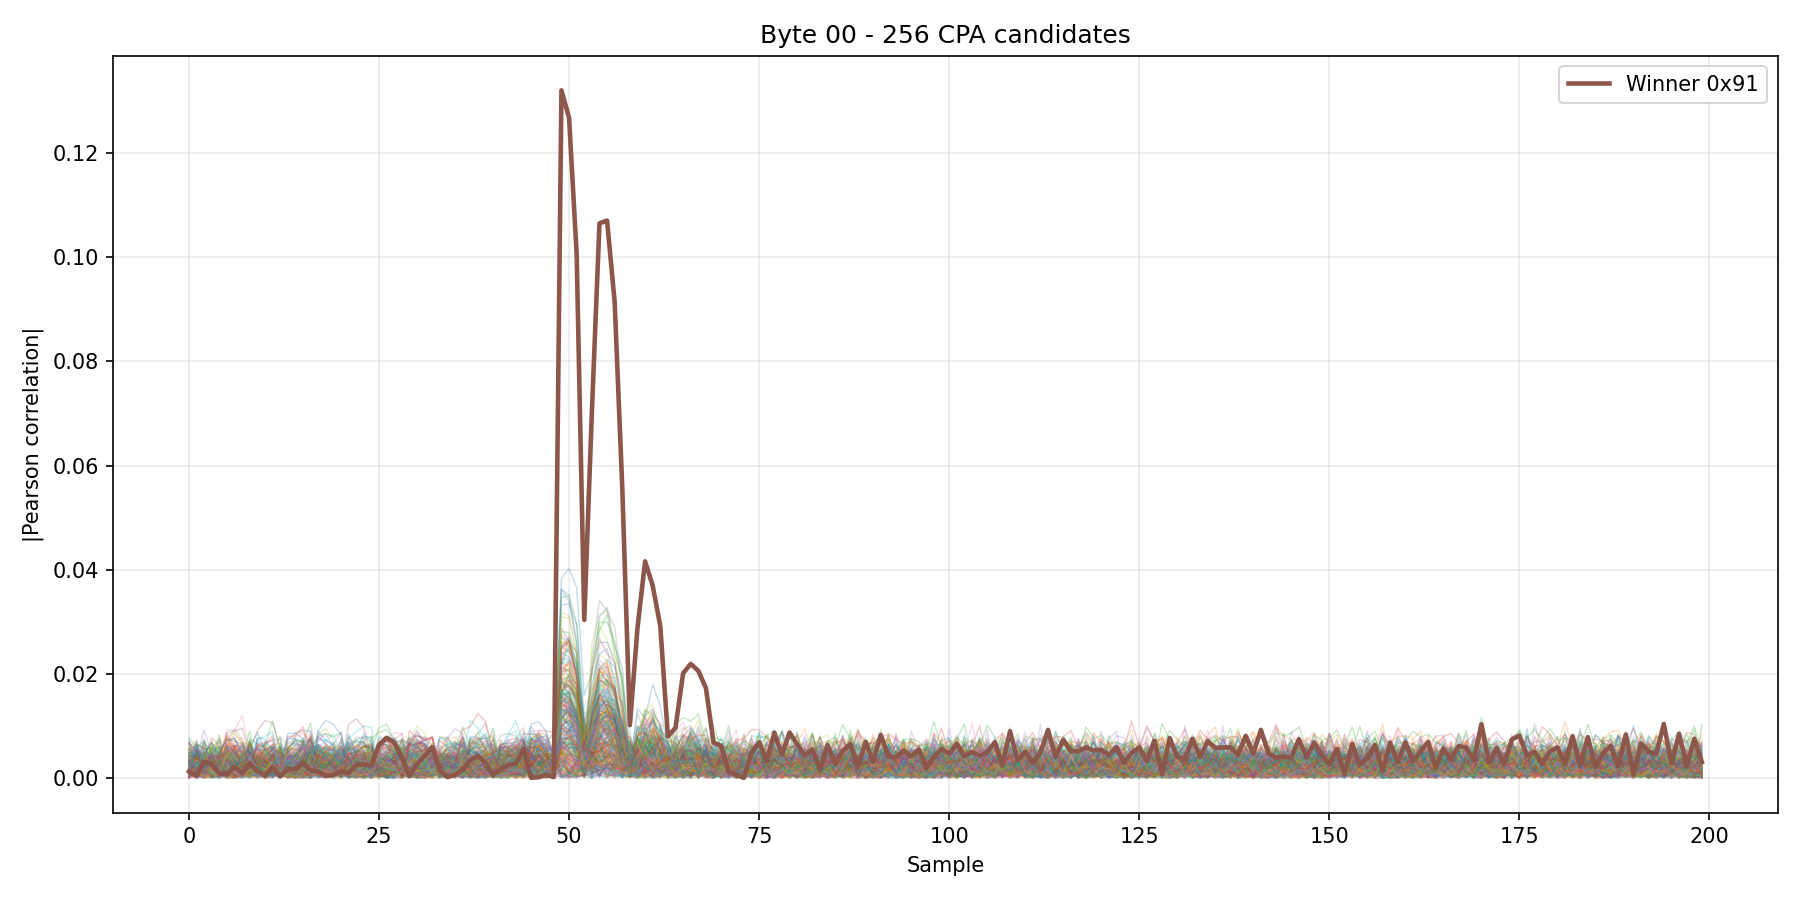
\includegraphics[width=0.92\textwidth]{correlation_plots_full/byte_00.png}
\caption{Task 1 example: absolute CPA correlations for the 256 guesses at byte 0.}
\label{fig:task1-example}
\end{figure*}

\subsection{Task 2: Number of Traces}
In the saved characterization, the first tested prefix with rank one for all 16 bytes contains 1,933 traces. Rank one is then observed for 100 consecutive tested counts beginning at 2,020. The earlier full-recovery point is a useful observed threshold for this ordering, while 2,020 is the more conservative stable threshold under the script's 100-count rule.

\begin{figure*}[t]
\centering
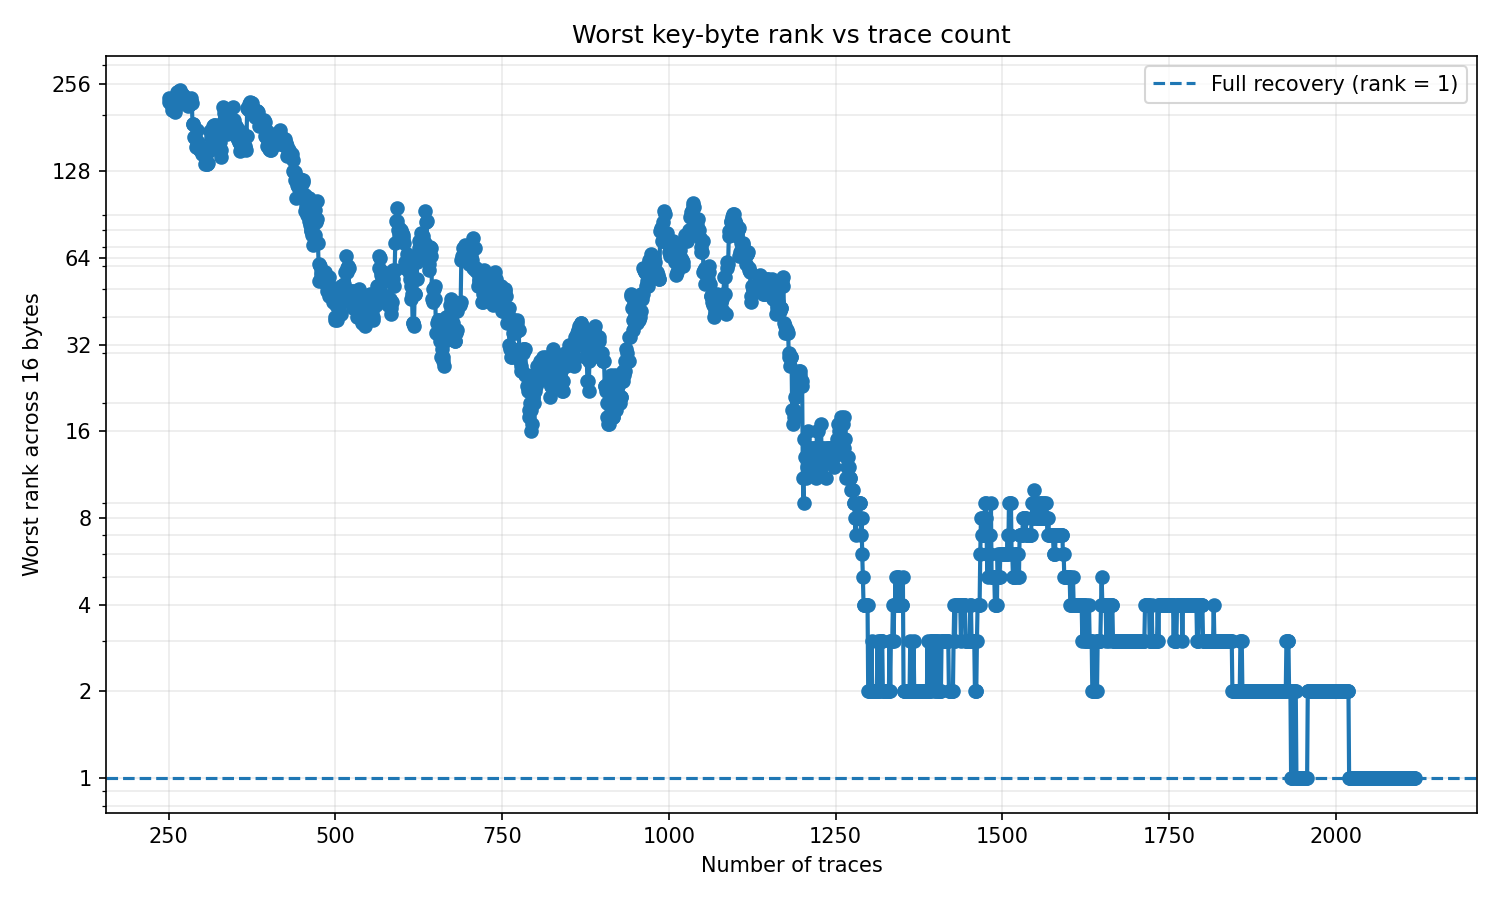
\includegraphics[width=0.86\textwidth]{worst_rank_plot.png}
\caption{Worst reference-key-byte rank as the number of traces increases. Rank one means all 16 reference bytes rank first.}
\label{fig:task2-worst-rank}
\end{figure*}

\begin{figure*}[t]
\centering
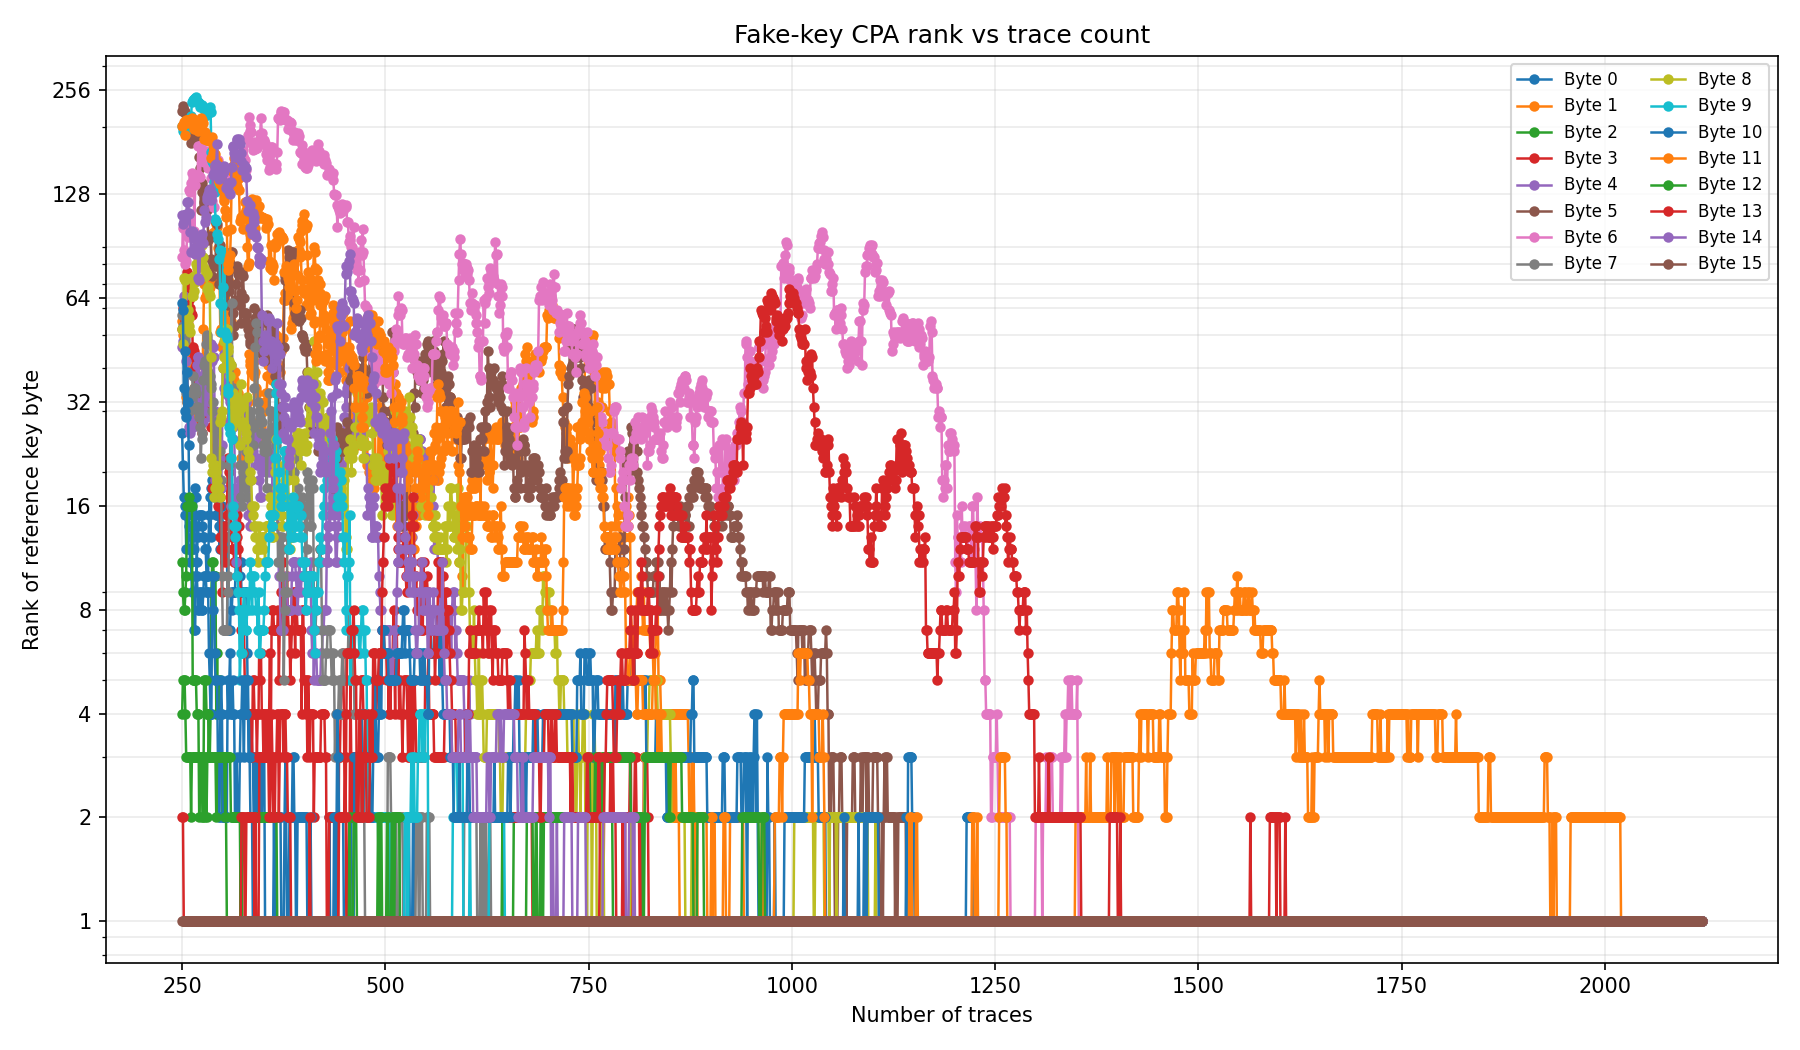
\includegraphics[width=0.92\textwidth]{rank_plot_all_bytes.png}
\caption{Reference-key-byte ranks across the tested trace counts.}
\label{fig:task2-byte-ranks}
\end{figure*}

\subsection{Task 3: Actual Round-10 Key}
The relation in Equation~\eqref{eq:doubled-fake-relation} links each doubled ciphertext value to its Task 1 fake key byte through $SBox(0)=\texttt{0x63}$. We used this repeated pattern as evidence of a lookup-table artifact. It motivated us to test a related but separate assumption for the absent values: one missing S-box input $z$ is shared across byte positions. This gives a manageable, testable set of 256 round-key candidates through Equation~\eqref{eq:rk10-candidates}. However, it is not a mathematical consequence of the doubled-value relation and histogram alone cannot distinguish all candidates. Both $z=0$ and $z=0\mathrm{xFF}$ remain possible at that stage.

The variance profile in Fig.~\ref{fig:variance} has ten selected local maxima at samples 13, 17, 21, 25, 29, 33, 37, 41, 45, and 49. Correlations for candidate transition features at the first eight event samples rank $z=0\mathrm{xFF}$ first. This gives the round-10 key candidate
\begin{equation*}
\texttt{d0\,14\,f9\,a8\,c9\,ee\,25\,89\,e1\,3f\,0c\,c8\,b6\,63\,0c\,a6}.
\end{equation*}

Figure~\ref{fig:task3-example} shows the candidate-correlation plots for byte 0 across rounds 1--8; the other 15 byte plots are supplied separately. These plots help inspect whether candidate peaks occur near the detected event samples. The numerical selection criterion is the aggregate score in Equation~\eqref{eq:endpoint-score}.

\begin{figure*}[!t]
\centering
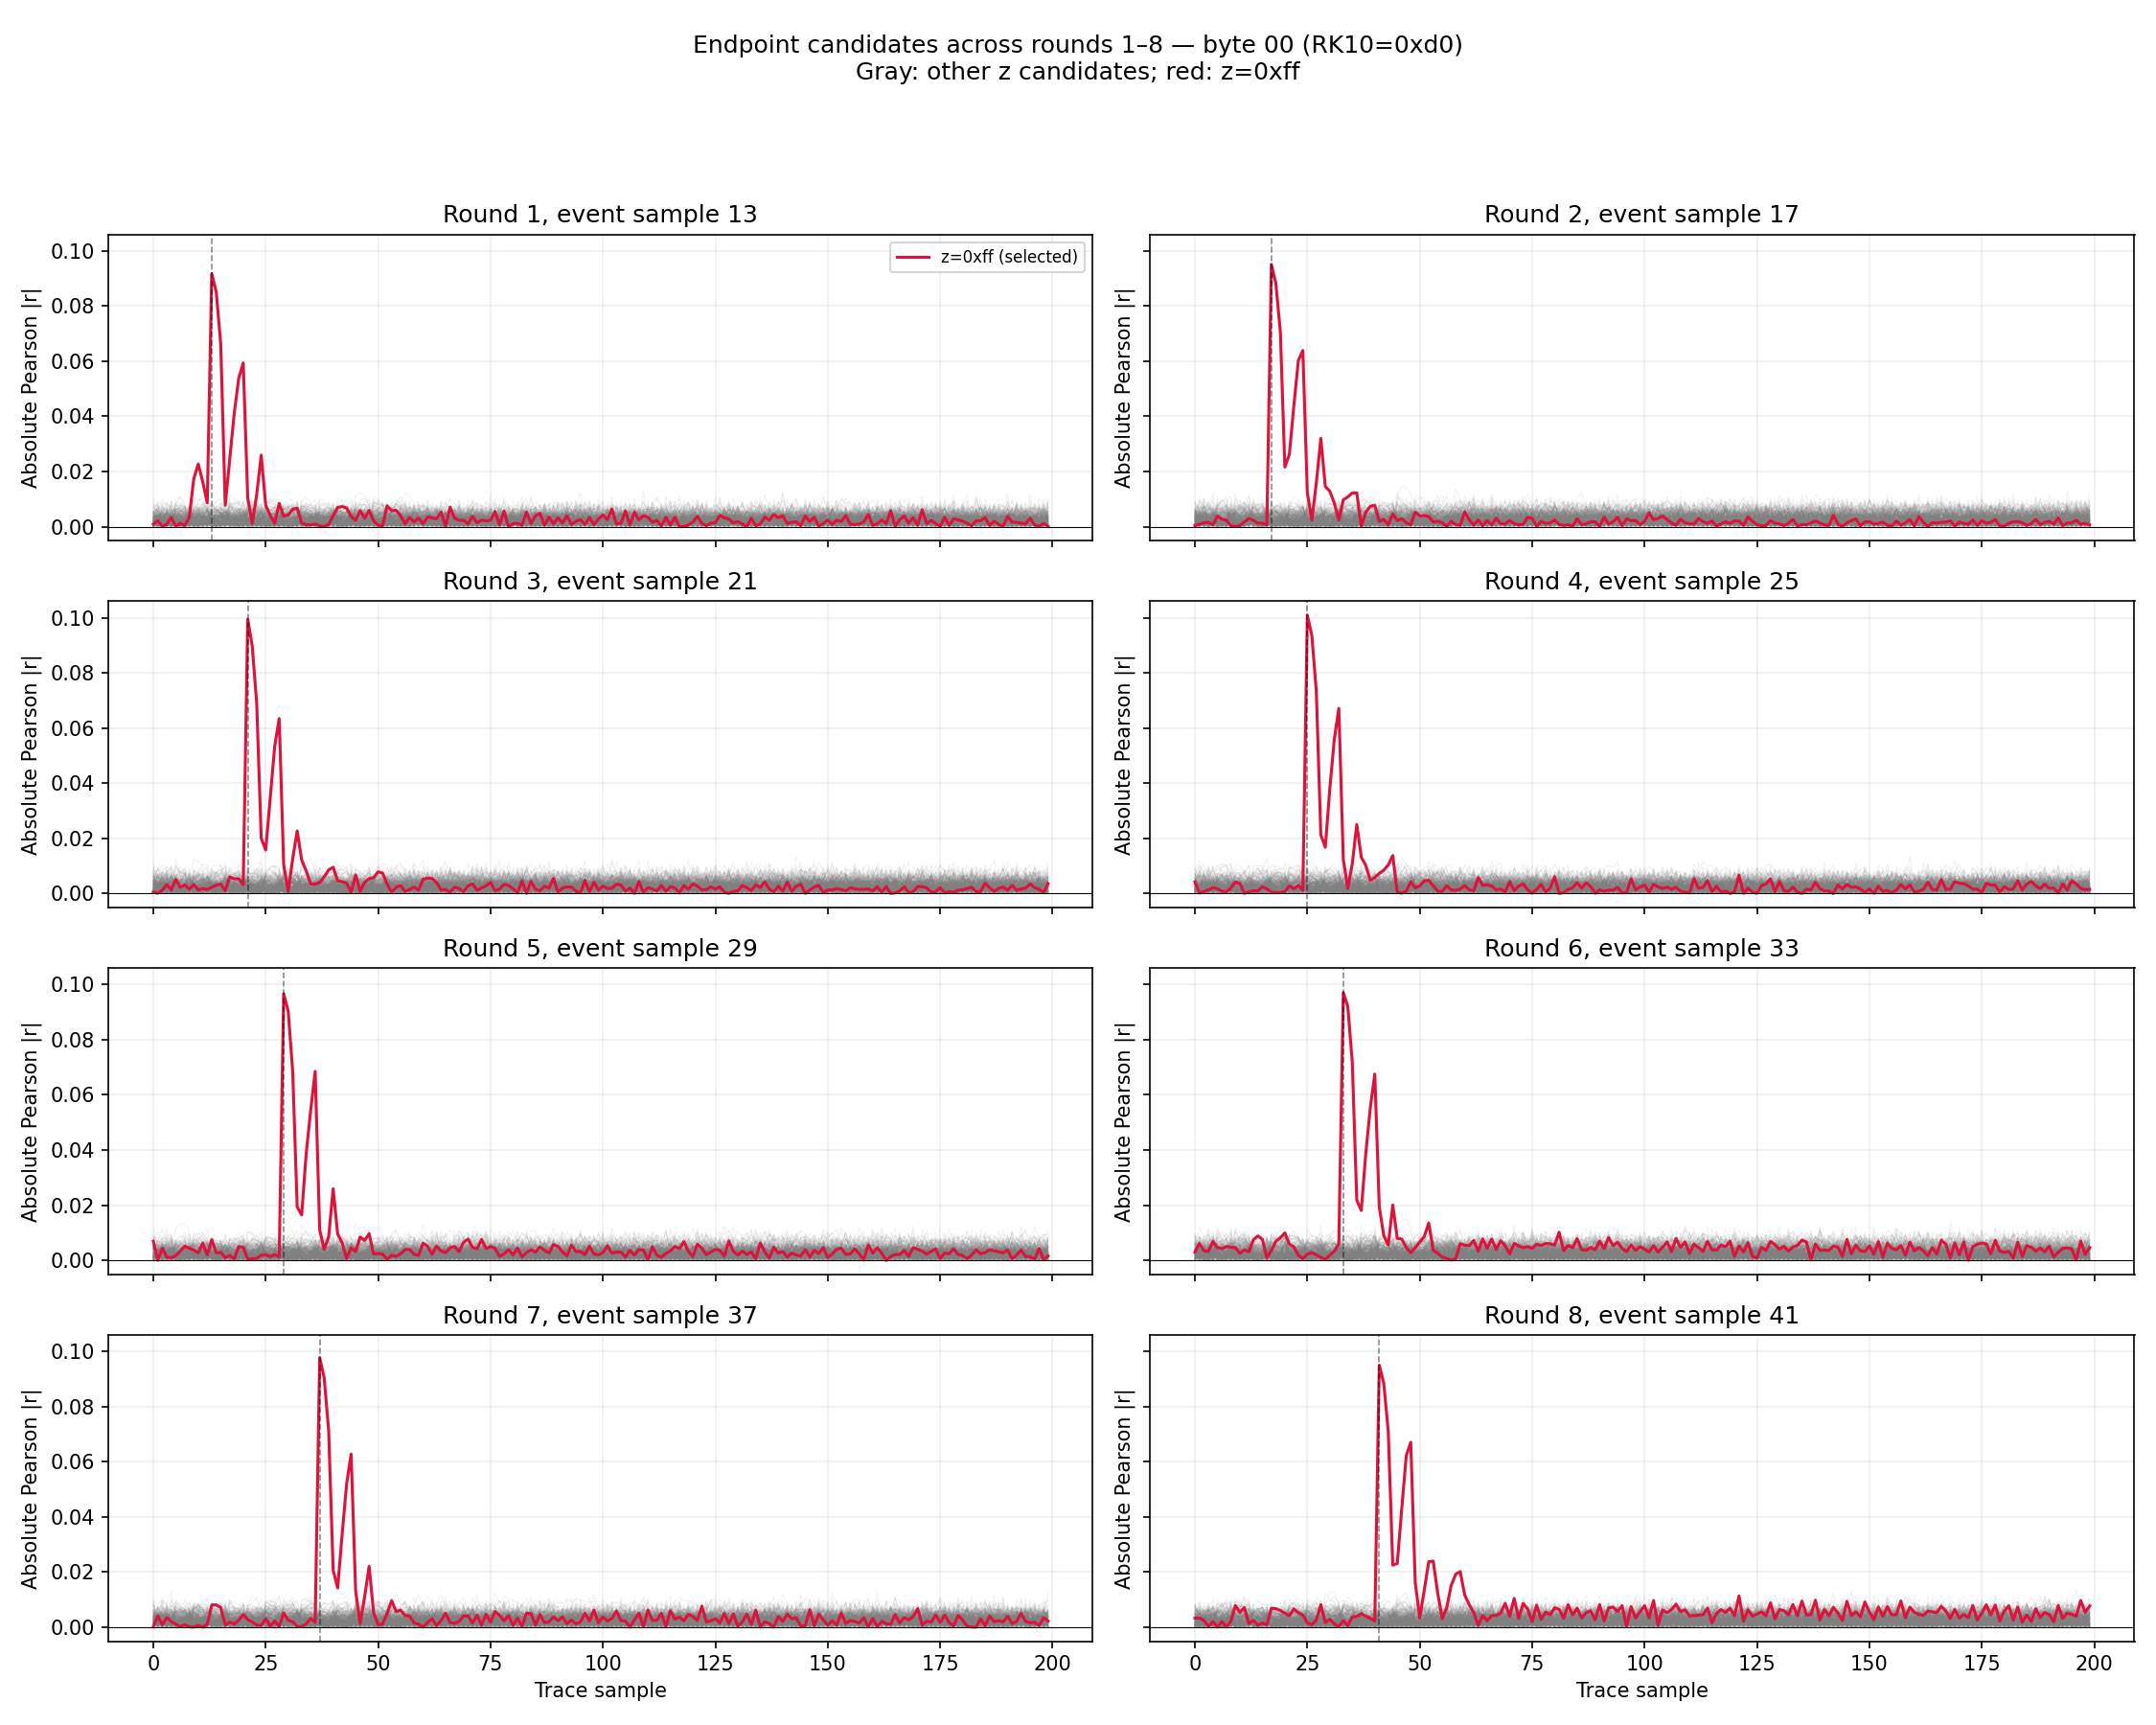
\includegraphics[width=0.96\textwidth]{actual_round10_correlation_plots/byte_00.png}
\caption{Task 3 example: endpoint-candidate correlations for byte 0 across rounds 1--8.}
\label{fig:task3-example}
\end{figure*}

\subsection{Task 4: AES-128 Master Key}
Starting with the round-10 key selected in Task 3, \texttt{fourth\_task.py} applies Equation~\eqref{eq:backward-schedule} until it reaches the first four words of the expanded key. Joining those words gives the master-key candidate
\begin{equation*}
\texttt{2b\,7e\,15\,16\,28\,ae\,d2\,a6\,ab\,f7\,15\,88\,09\,cf\,4f\,3c}.
\end{equation*}
The script checks this result by generating all the round keys again from the recovered master key. Its round-10 output is \texttt{d014f9a8c9ee2589e13f0cc8b6630ca6}, which matches the key supplied by Task 3.

This check confirms that the recovered master key corresponds to the selected round-10 key. Since possible 128-bit round key leads to a corresponding AES-128 master key when we reverse the schedule, we therefore use the trace analysis in Task 3 to support the key selection, and the forward expansion check in Task 4 to support the calculation.

\begin{table}[t]
\caption{Summary of the four task results}
\label{tab:summary}
\centering
\footnotesize
\begin{tabularx}{\columnwidth}{@{}c>{\raggedright\arraybackslash}p{0.25\columnwidth}>{\raggedright\arraybackslash}X@{}}
\toprule
Task & Target & Result \\
\midrule
1 & Fake round-10 key & \texttt{91dec068e3face45}\newline\texttt{99ce38f420863a30} \\
2 & Trace count & First full recovery: 1,933; stable 100-count run begins: 2,020 \\
3 & Actual round-10 key & \texttt{d014f9a8c9ee2589}\newline\texttt{e13f0cc8b6630ca6}; selected $z=0\mathrm{xFF}$ \\
4 & AES-128 master key & \texttt{2b7e151628aed2a6}\newline\texttt{abf7158809cf4f3c} \\
\bottomrule
\end{tabularx}
\end{table}

\section{Limitations}

Task 2 conclusion is dependent on the random seed, which is included to counter the ordering of traces. If the seed is changed the minimum number of traces might differ.

Task 3 conclusion depends on several assumptions: the same missing S-box input applies to all 16 byte positions; retained rows correspond to standard AES encryptions; the selected variance peaks correspond to AES round events; and ordinary-round leakage is sufficiently described by transition Hamming distance.

Task 4 starts with the round-10 key that Task 3 selects for $z=\texttt{0xFF}$. Once we choose that round key, the backward calculation gives one corresponding master key. Expanding it forward checks that we have performed the key-schedule calculation correctly. The evidence that this is the device's actual key still comes from Task 3 and depends on the assumptions listed above.

\section{Conclusion}
CPA over the final-round transition model recovers the fake round-10 key, and a rank characteristics shows how that reference key performs as the trace count grows. Ciphertext-frequency observations then provide a set of actual round-key candidates, while earlier-round transition correlations favor the shared endpoint $z=0\mathrm{xFF}$. Reversing the calculated RK10 derived from z values gives the corresponding master-key candidate. The fake key result follows directly from the stated CPA ranking; the actual-key result is shown probable by using correlation plots.

\clearpage
\begin{thebibliography}{7}
\raggedright
\def\UrlBreaks{\do\/\do\.\do\-}
\bibitem{kocher}
P. C. Kocher, J. Jaffe, and B. Jun, ``Differential power analysis,'' in \emph{Advances in Cryptology---CRYPTO '99}, Lecture Notes in Computer Science, vol. 1666. Berlin, Germany: Springer, 1999, pp. 388--397.

\bibitem{brier}
E. Brier, C. Clavier, and F. Olivier, ``Correlation power analysis with a leakage model,'' in \emph{Cryptographic Hardware and Embedded Systems---CHES 2004}, Lecture Notes in Computer Science, vol. 3156. Berlin, Germany: Springer, 2004, pp. 16--29.

\bibitem{oflynn2014}
C. O'Flynn and Z. Chen, ``Side Channel Power Analysis of an AES-256 Bootloader,'' \emph{Cryptology ePrint Archive}, Paper 2014/899, 2014. [Online]. Available: \url{https://eprint.iacr.org/2014/899}

\bibitem{faking}
R. Lumbiarres-L\'opez, M. L\'opez-Garc\'ia, and E. Cant\'o-Navarro, ``Faking countermeasure against side-channel attacks,'' in \emph{Advances in Microelectronics: Reviews}, vol. 1, S. Y. Yurish, Ed. IFSA Publishing, 2017, ch. 19, pp. 509--526. [Online]. Available: \url{https://upcommons.upc.edu/server/api/core/bitstreams/522a48dd-2d29-4aee-9395-aa70b82008a8/content}

\bibitem{novak-reverse}
R. Novak, ``Side-channel based reverse engineering of secret algorithms,'' in \emph{Proceedings of the 12th International Electrotechnical and Computer Science Conference (ERK 2003)}, 2003, pp. 445--448. [Online]. Available: \url{https://www.researchgate.net/publication/228847690_Side-channel_based_reverse_engineering_of_secret_algorithms}

\bibitem{fips197}
National Institute of Standards and Technology, \emph{Advanced Encryption Standard (AES)}, FIPS PUB 197-upd1, May 2023. [Online]. Available: \url{https://doi.org/10.6028/NIST.FIPS.197-upd1}

\bibitem{cse-inversion}
poncho, ``Answer to: In AES keyschedule, infer all round keys and cipher key from last round key,'' \emph{Cryptography Stack Exchange}, Jul. 31, 2017, edited Aug. 1, 2017. [Online]. Available: \url{https://crypto.stackexchange.com/questions/50543/in-aes-keyschedule-infer-all-round-keys-and-cipher-key-from-last-round-key}

\end{thebibliography}
\end{document}

